\subsubsection{Influence}

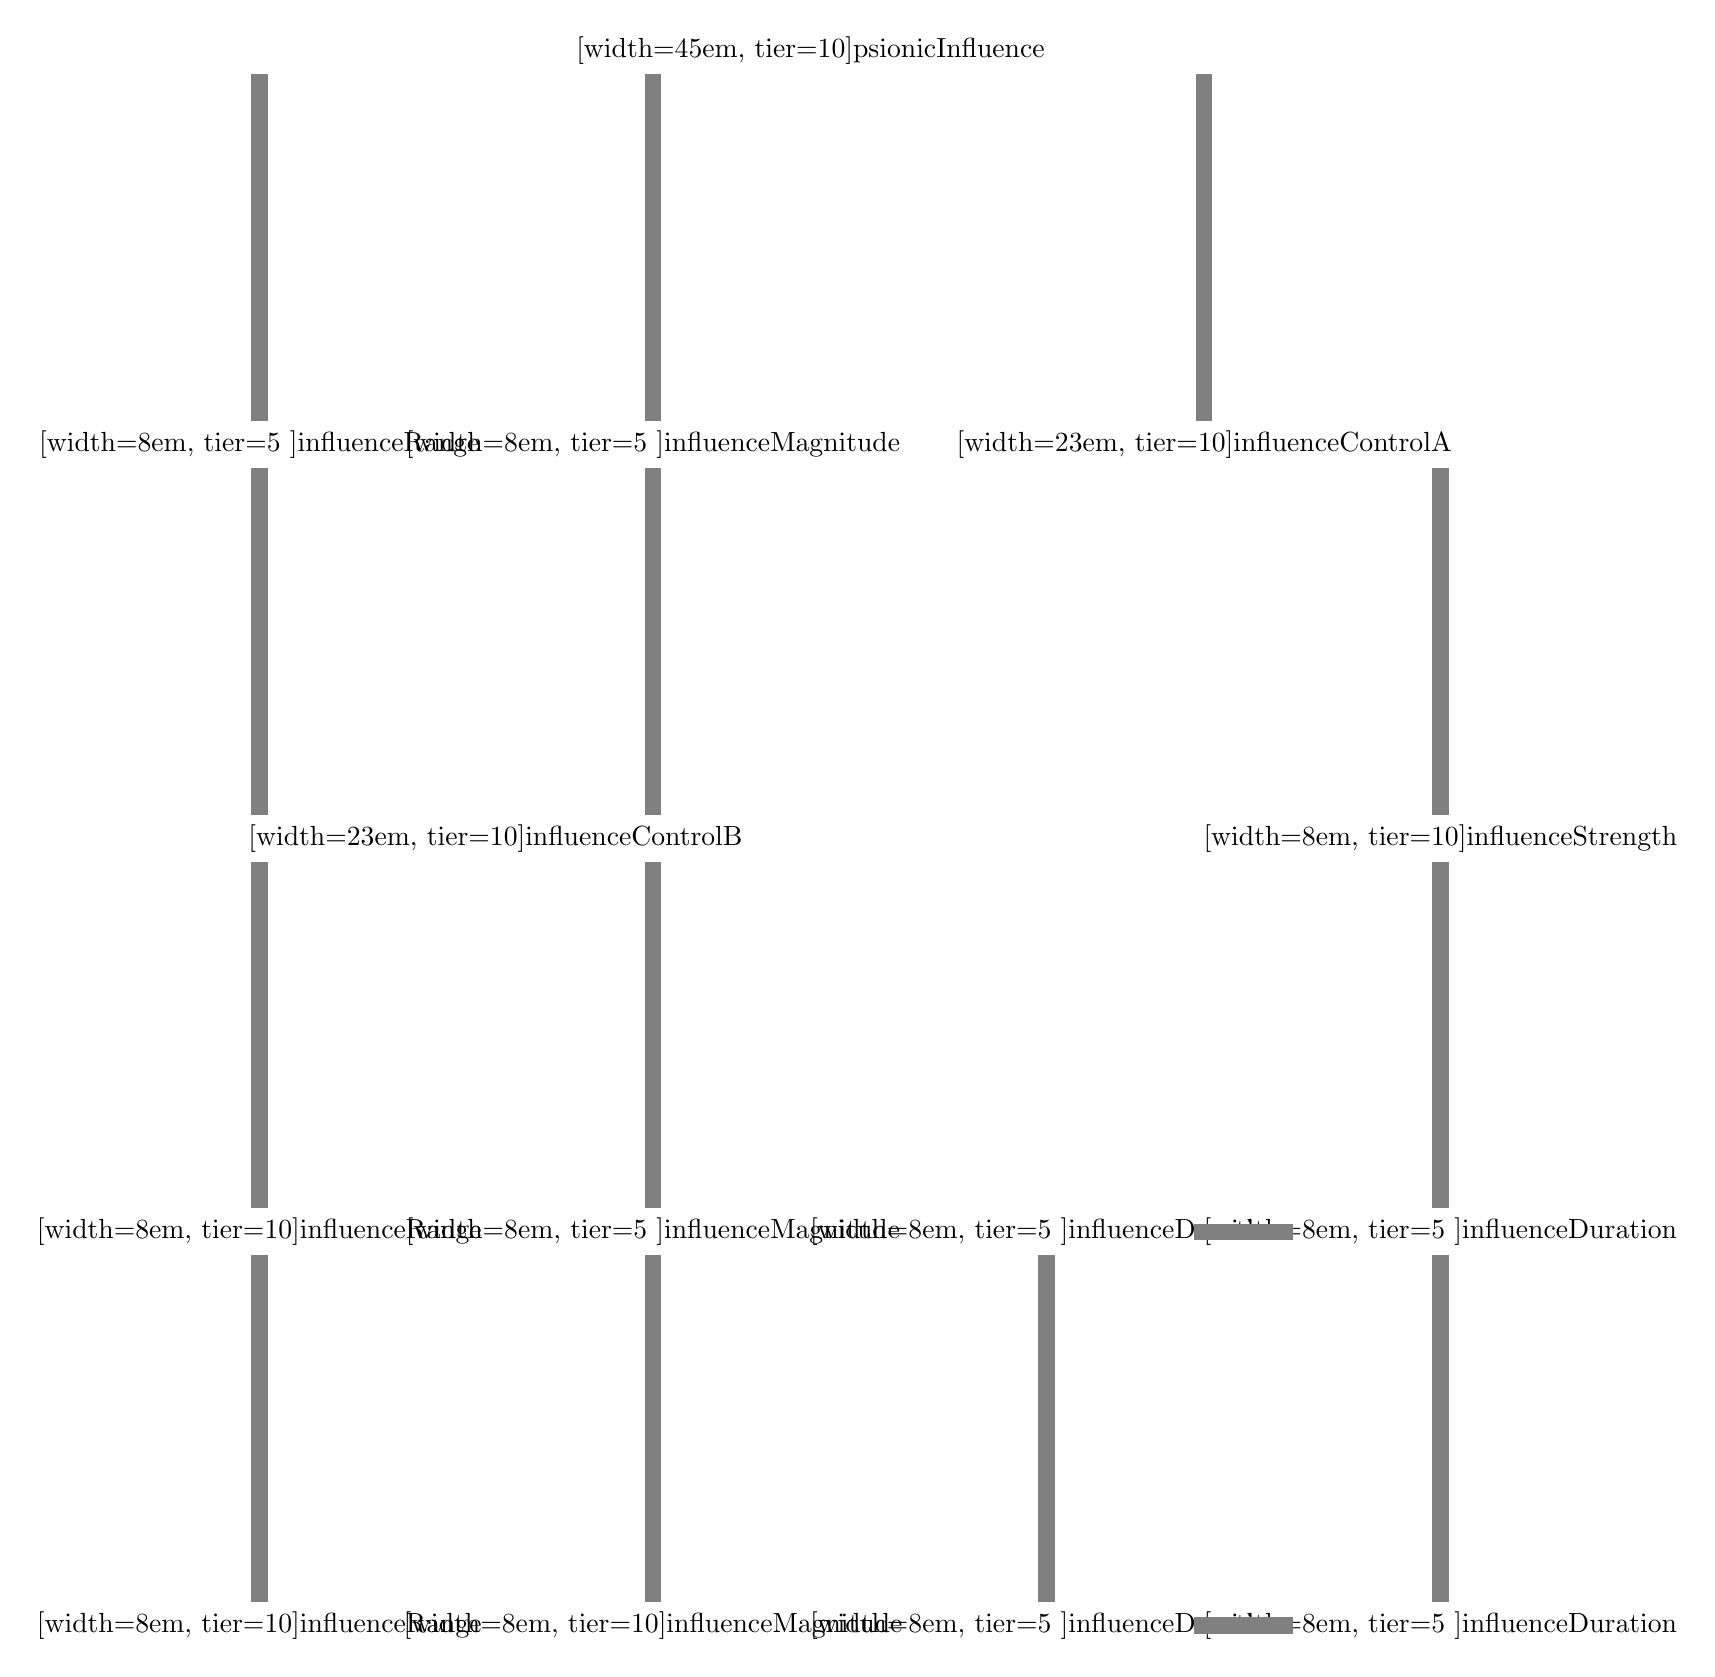
\begin{tikzpicture}
    \draw (-13,  -2) node(pr){\TalentBox[width=45em, tier=10]{psionicInfluence}};
    \draw (-20,  -7) node(aa){\TalentBox[width=8em,  tier=5 ]{influenceRange}}
          (-15,  -7) node(ab){\TalentBox[width=8em,  tier=5 ]{influenceMagnitude}}
          ( -8,  -7) node(ad){\TalentBox[width=23em, tier=10]{influenceControlA}}
          (-17, -12) node(bb){\TalentBox[width=23em, tier=10]{influenceControlB}}
          ( -5, -12) node(bd){\TalentBox[width=8em,  tier=10]{influenceStrength}}
          (-20, -17) node(ca){\TalentBox[width=8em,  tier=10]{influenceRange}}
          (-15, -17) node(cb){\TalentBox[width=8em,  tier=5 ]{influenceMagnitude}}
          (-10, -17) node(cc){\TalentBox[width=8em,  tier=5 ]{influenceDuration}}
          ( -5, -17) node(cd){\TalentBox[width=8em,  tier=5 ]{influenceDuration}}
          (-20, -22) node(da){\TalentBox[width=8em,  tier=10]{influenceRange}}
          (-15, -22) node(db){\TalentBox[width=8em,  tier=10]{influenceMagnitude}}
          (-10, -22) node(dc){\TalentBox[width=8em,  tier=5 ]{influenceDuration}}
          ( -5, -22) node(dd){\TalentBox[width=8em,  tier=5 ]{influenceDuration}}
    ;

    \tikzstyle{bar}=[gray,-,>=stealth, line width=6pt]

    \draw [bar] (aa) -- (aa |- pr.south);
    \draw [bar] (ab) -- (ab |- pr.south);
    \draw [bar] (ad) -- (ad |- pr.south);
    \draw [bar] (aa) -- (aa |- bb.north);
    \draw [bar] (ab) -- (ab |- bb.north);
    \draw [bar] (bd) -- (bd |- ad.south);
    \draw [bar] (ca) -- (ca |- bb.south);
    \draw [bar] (cb) -- (cb |- bb.south);
    \draw [bar] (bd) edge (cd);
    \draw [bar] (ca) edge (da);
    \draw [bar] (cb) edge (db);
    \draw [bar] (cc) edge (dc);
    \draw [bar] (cc) edge (cd);
    \draw [bar] (cd) edge (dd);
    \draw [bar] (dc) edge (dd);
\end{tikzpicture}
